\documentclass[12pt,a4paper]{article}
\usepackage[natbibapa]{apacite}
\usepackage{graphicx}
\usepackage{amsmath}
\usepackage{geometry}
\usepackage{setspace}
\usepackage{enumitem}
\usepackage{hyperref} 
\usepackage{lipsum}
% Page setup
\geometry{margin=1in}
\setstretch{1.5}

% Title Page
\title{Research Proposal  on [The Role of Artificial Intelligence in Enhancing Software Testing]}
\author{Group Members: \\
\textbf{CHIN ZHEN HO (1221102540)} \\
\textbf{ERIC TEOH WEI XIANG (1221102007)} \\
\textbf{BERNARD RYAN SIM KANG XUAN (1221101777)} \\
\textbf{GAN SHAO YANG (1221103201)} \\
\\
Course: Research Methodologies for Computer Science \\
Assignment 2 - Research Proposal  \\
Date of Submission: [ 25th September 2024 ]}
\date{}

\begin{document}

\maketitle
\newpage


% Table of Contents
\tableofcontents
\newpage

% 1. Executive Summary
\section{Executive Summary}

    Current AI-driven software testing tools, particularly those leveraging Large Language Models (LLMs), face several challenges. These include inconsistent performance across different programming languages, limited automation capabilities in integration testing, and insufficient frameworks for testing AI/ML models, especially in addressing issues like overfitting and algorithmic uncertainty.\\

    The main objectives of this research are to evaluate the reliability of LLM-generated unit tests across multiple programming languages, explore the use of AI tools to automate complex integration testing, and develop specialized testing frameworks for AI/ML models to tackle overfitting and uncertainty issues.\\

    The research will employ a combination of empirical experiments and comparative analyses. It will assess the reliability of LLM-generated unit tests in diverse programming languages, implement and test AI tools in integration scenarios, and design new frameworks to address challenges in testing AI/ML systems. Performance will be evaluated based on metrics such as test accuracy, coverage, and error detection.\\

    The expected outcomes of this research include the establishment of standardized methodologies for generating unit tests across various programming languages, the development of improved tools for automating integration testing, and the creation of robust testing frameworks for AI/ML models. These advancements are anticipated to significantly enhance the scalability, efficiency, and accuracy of AI-driven testing processes, leading to more reliable software systems in industries such as finance, healthcare, and autonomous systems.
\begin{itemize} 
    \item \textbf{Keywords:} Artificial Intelligence, Large Language Models, Software Testing, Integration Testing, AI/ML Models, Overfitting, Algorithmic Uncertainty, Automation, Unit Testing, Testing Frameworks
\end{itemize}

% 2.  Introduction
\section{ Introduction}

\begin{itemize}
    \item \textbf{Background:}  As software systems grow in complexity and the demand for rapid development cycles increases, traditional manual software testing methods have become inefficient and error-prone. Artificial Intelligence (AI), particularly in the form of LLMs such as GPT-3.5 and GPT-4, holds significant potential for automating and improving software testing. Despite these advancements, AI-driven testing tools face critical challenges, such as limited reliability across programming languages, inadequate support for complex integration testing, and difficulties in testing AI/ML models that exhibit unpredictable behavior.

    \item \textbf{Research Topic:} This proposal explores how AI-driven tools can be optimized to address the current limitations in software testing by improving reliability, scalability, and adaptability in diverse testing environments.

    \item \textbf{Importance:} Addressing these challenges is crucial for enhancing the accuracy, speed, and reliability of software testing processes, which are foundational to ensuring the development of robust and error-free software in various high-stakes industries.
\end{itemize}
\newpage

% 3. Problem Statement with Justification/Motivation
\section{Problem Statement with Justification/Motivation}

\begin{itemize}
    \item \textbf{Problem 1: Inconsistent performance of LLM-generated unit tests across programming languages.} \\
     Existing research, such as that focused on GPT-3.5, has primarily explored the application of LLMs in generating unit tests for a single programming language, usually Java. This narrow scope limits the generalizability of AI-based testing tools to other programming languages commonly used in software development, such as Python, C++, and JavaScript.
    \begin{itemize}
    \item \textbf{Justification:} Establishing the reliability of LLMs across multiple languages will provide developers with more versatile AI-driven tools, enabling broader adoption of AI-based unit testing across the software industry.
    \end{itemize}
 
    \item \textbf{Problem 2: Limited AI support for automating integration testing. }\\
    While AI has made strides in automating unit and regression testing, integration testing—where multiple software components are tested together to ensure they interact correctly—remains relatively unexplored by AI-driven tools. Integration testing is complex, requiring the coordination of different subsystems, and manual testing is time-consuming and prone to errors.
    \begin{itemize}
    \item \textbf{Justification:} Automating integration testing with AI would significantly reduce the manual effort involved and improve overall system robustness, enabling quicker and more reliable software releases.
    \end{itemize}

    \item \textbf{Problem 3: Challenges in testing AI/ML models due to overfitting and algorithmic uncertainty. }\\
    Traditional software testing methods are ill-equipped to handle the dynamic and unpredictable behavior of AI/ML systems, which often suffer from issues like overfitting (where a model performs well on training data but poorly on new data) and incomprehensible decision-making processes.
    \begin{itemize}
    \item \textbf{Justification:} Developing specialized testing frameworks for AI/ML models is essential to ensure their reliability in real-world applications, particularly in critical sectors like autonomous systems and healthcare, where the consequences of faulty AI behavior can be severe.

    \end{itemize}
    
\end{itemize}

\newpage
% 4. Research Questions, Hypotheses, and Research Objectives
\section{Research Questions, Hypotheses, and Objectives}
\begin{itemize}
    \item \textbf{Research Questions:} 
    \begin{enumerate}
    \item How reliable are LLMs, such as GPT-4, in generating unit tests for different programming languages?
    \item Can AI-driven tools effectively automate integration testing, and how do they compare with traditional manual methods in terms of accuracy and efficiency?
    \item What specialized frameworks can be developed to improve the testing of AI/ML models, particularly in mitigating issues related to overfitting and algorithmic uncertainty?
    \end{enumerate}

    \item \textbf{Hypotheses:} 
    \begin{enumerate}
    \item LLM-generated unit tests, when appropriately fine-tuned, will perform reliably across a variety of programming languages.
    \item AI-driven tools can automate integration testing more efficiently and accurately than traditional manual approaches.
    \item New testing frameworks designed for AI/ML systems will improve the models' generalizability and robustness, reducing overfitting and enhancing performance in real-world scenarios.
    \end{enumerate}
    
    \item \textbf{Research Objectives:} 
    \begin{enumerate}
    \item To empirically evaluate the performance of LLMs in generating unit tests across diverse programming languages.
    \item To design and implement AI-driven tools for automating integration testing, and assess their effectiveness compared to manual methods.
    \item To develop and validate specialized testing frameworks for AI/ML systems that address overfitting and uncertainty.
    \end{enumerate}

\end{itemize}
\newpage
% 5. Literature Review Summary
\section{Literature Review Summary}
 
     The current body of research on AI-driven software testing, particularly with the use of Large Language Models (LLMs) like GPT-3.5 and GPT-4, reveals both significant advancements and critical gaps. A common theme in the literature is the exploration of LLMs for unit test generation. \citep{Guilherme23} demonstrated that GPT-3.5 can generate unit tests for Java programs, and while these tests can be effective, their performance is often inconsistent and heavily influenced by fine-tuning factors such as temperature settings. This limitation points to the need for more robust methods that ensure consistent results across varying environments. Similarly,\citep{Boukhlif24} emphasize the importance of prompt engineering and the need for model fine-tuning to achieve reliable outcomes from LLMs. While these studies underscore the potential of LLMs to automate certain aspects of testing, they also highlight the limitations in achieving consistent and scalable results without extensive customization.

     Another recurring theme is the automation of testing processes at various stages of software development, with \citep{Minimol21} noting the substantial impact AI-driven tools such as Selenium and Testim have had in automating regression and UI testing. These tools significantly reduce the manual effort required and improve accuracy. However, despite these advancements, integration testing—a more complex process that involves ensuring the proper interaction of multiple software components—remains relatively unexplored in AI-driven frameworks. This gap suggests that while AI has improved specific types of testing, its application in more comprehensive and integrative scenarios is still underdeveloped \citep{Minimol21}.


   The testing of AI/ML models presents another significant challenge. \citep{Kishore21} identify critical issues such as overfitting and algorithmic uncertainty that traditional testing methods are ill-equipped to handle. AI/ML models, by their nature, require new testing frameworks that can address their dynamic behavior, ensuring they generalize well to new data and perform reliably in real-world scenarios. The lack of such specialized frameworks highlights an important gap in the current research, especially given the growing reliance on AI/ML systems in critical sectors such as healthcare and autonomous vehicles \citep{Kishore21}.

Despite the promising advancements, several gaps remain in the literature. One major gap is the lack of research into the cross-language applicability of LLMs for unit test generation. Most studies, like those by \citep{Guilherme23}, focus on a single language, typically Java, without exploring the performance of LLMs across other programming languages such as Python, C++, or JavaScript. Another key gap is the limited exploration of AI-driven integration testing. While tools like Selenium have been highly effective in specific testing areas, their application in automating integration testing remains underexplored \citep{Minimol21}. Lastly, the literature underscores the need for specialized frameworks designed specifically for testing AI/ML models, which are currently absent but essential for addressing issues like overfitting and algorithmic uncertainty \citep{Kishore21}. Future research must address these gaps by developing more generalized LLM tools that work across different languages, automating more complex testing processes such as integration, and creating frameworks tailored for the unique challenges posed by AI/ML systems.



% 6. Research Methodology
\section{Research Methodology}
\begin{itemize}
    \item \textbf{Step 1: Empirical Evaluation of LLM-Generated Unit Tests Across Multiple Programming Languages}\\
    Select LLM models (e.g., GPT-4, Codex) and fine-tune them for unit test generation in Java, Python, and C++. Generate tests for diverse software programs, evaluating effectiveness using metrics like code coverage, fault detection rates, and mutation scores. Compare LLM-generated tests against traditional tools like EvoSuite. Explore variations in performance by adjusting input parameters.
    
    \item \textbf{Step 2: Development and Evaluation of AI-Driven Integration Testing Tools} \\
    Review and select existing AI tools (e.g., Selenium, Testim) compatible with the experimental environment. Automate complex integration scenarios involving databases and APIs, creating customized test cases. Conduct a comparative analysis with manual tests, measuring test accuracy, time efficiency, error reduction, and scalability.
    
    \item \textbf{Step 3: Designing Specialized Frameworks for AI/ML System Testing}\\
    Design frameworks addressing challenges like overfitting and algorithmic uncertainty for AI/ML systems. Test these frameworks on real-world models to evaluate their robustness and generalization capabilities. Use case studies from industries such as healthcare to validate applicability.

    \item \textbf{Metrics:} Key performance indicators (KPIs) for this research will include:
    \begin{itemize}
    \item \textbf{Code Coverage:} The percentage of the software's code that is executed by the tests.

    \item \textbf{Test Accuracy:} The ability of the AI-driven tools to detect actual faults within the software.

    \item \textbf{Fault Detection Rate:} The number of errors identified by the tests compared to known faults.

    \item \textbf{Reduction of Overfitting:} The ability of AI/ML testing frameworks to reduce model overfitting, measured by the generalization of AI models on new, unseen data.

    \item \textbf{Robustness:} The frameworks’ effectiveness in handling AI/ML models in complex and unpredictable real-world scenarios, such as autonomous vehicles or medical diagnostics.
    \end{itemize}

\end{itemize}
% 7. Research Activities and Milestones
\section{Research Activities and Milestones}
\begin{center}
\begin{tabular}{ |p{10cm}|p{5cm}|}
 \hline
 \multicolumn{2}{|c|}{Research Activities} \\
 \hline
 Activities & Month \\
 \hline
 Set up the experimental framework for comparative analysis of LLM-generated unit tests across different programming languages   & 1-2    \\
 \hline
 Conduct comparative analysis of LLM-generated unit tests across multiple programming languages. Measure performance using metrics such as code coverage, fault detection, and execution time. & 3-4 \\
 \hline
Begin implementation of AI-driven integration testing tools. Develop test cases for integration scenarios involving multiple software components. & 5-6 \\
\hline
Conduct experiments to compare AI-driven integration testing tools against traditional manual approaches. Collect performance metrics, including test accuracy, time efficiency, and error detection rates. & 7-8 \\
\hline
Develop specialized frameworks for testing AI/ML models, focusing on addressing challenges such as overfitting and algorithmic uncertainty. Prepare testing environments using real-world case studies. & 9-10 \\
\hline
Conduct preliminary testing of the developed frameworks on AI/ML models, using metrics such as generalization, robustness, and overfitting reduction. & 11 \\
\hline
 Finalize the specialized testing frameworks, complete data analysis from all experiments, and prepare research reports and documentation for publication. & 12 \\
 \hline 
\end{tabular}
\end{center}
\begin{figure}
    \centering
    \label{fig:Flowchart}
    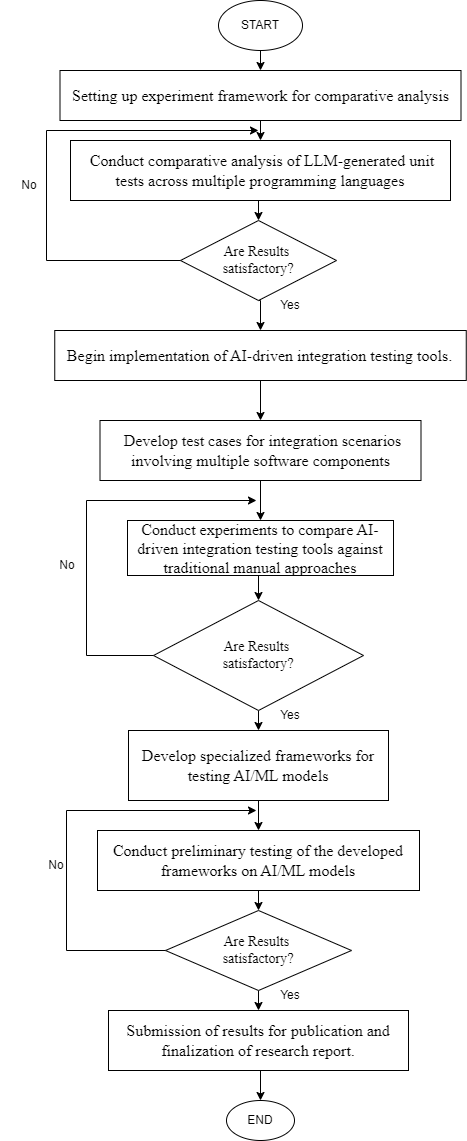
\includegraphics[width=0.5\linewidth]{research.drawio (1).png}
    \caption{Flowchart}
    
\end{figure}
\newpage

\begin{center}
\begin{tabular}{ |p{10cm}|p{5cm}|}
 \hline
 \multicolumn{2}{|c|}{Research Schedules} \\
 \hline
 Description & Month \\
 \hline
 Complete the experimental design and preparation of datasets for testing different programming languages.   & 1-2    \\
 \hline
Completion of initial LLM-generated test evaluation and data collection. & 3-4 \\
 \hline
Initial implementation of AI-driven tools for integration testing and setup of comparison with manual methods. & 5-6 \\
\hline
Completion of integration testing tool evaluation and analysis of results. & 7-8 \\
\hline
Framework development completed and initial testing environment prepared. & 9-10 \\
\hline
Completion of preliminary testing and initial results analysis. & 11 \\
\hline
Submission of results for publication and finalization of research report. & 12 \\
 \hline 
\end{tabular}
\end{center}
\begin{figure}
    \centering
    \label{fig:Gantt Chart}
    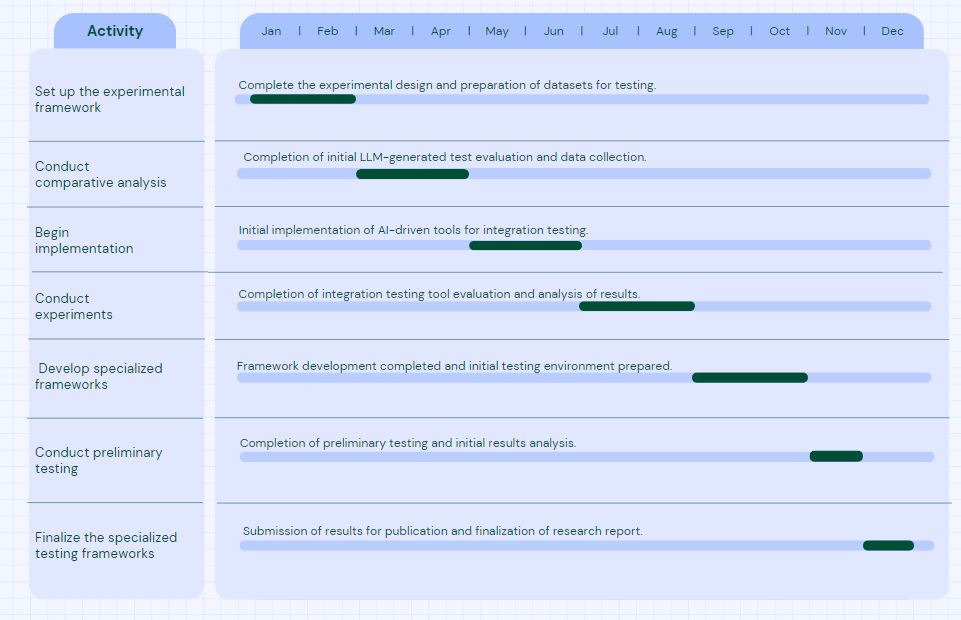
\includegraphics[width=1\linewidth]{Gantt Chart.png}
    \caption{Gantt Chart}
    
\end{figure}
\newpage



% 8. Expected Results and Impact
\section{Expected Results and Impact}
\begin{itemize}
    \item \textbf{Expected Results:}\\
    The research is expected to produce reliable, standardized methods for generating unit tests across multiple programming languages, AI-driven tools for automating integration testing, and specialized frameworks for testing AI/ML models. These contributions will address key gaps in current software testing practices and significantly improve testing efficiency, accuracy, and scalability.

    \item \textbf{Impact:}\\
     The outcomes will have far-reaching implications across various industries, particularly those that rely heavily on complex software systems and AI/ML models, such as autonomous vehicles, healthcare, and financial services. By improving the reliability and efficiency of software testing, this research will contribute to higher software quality, reduced development costs, and faster time-to-market for software solutions.


\end{itemize}

% References
\newpage
\bibliographystyle{apacite} % Choose the appropriate bibliography style (e.g., APA, IEEE)
\bibliography{MyBib}{} % Make sure to include a MyBib.bib file with your references

% Appendices (if necessary)
\appendix
\section{Appendix A: Member Contributions}
\begin{table}[h]
    \centering
    \begin{tabular}{|c|c|c|}
        \hline
        Student Name & Student ID & Contribution percentages \\
        \hline
        CHIN ZHEN HO & 1221102540 & 25\% \\
        \hline
        ERIC TEOH WEI XIANG & 1221102007 & 25\% \\
        \hline
        BERNARD RYAN SIM KANG XUAN & 1221101777 & 25\% \\
        \hline
        GAN SHAO YANG & 1221103201 & 25\% \\
        \hline

    \end{tabular}
    \caption{Members Contribution Table}
    \label{tab:my_label}
\end{table}


\end{document}

